\documentclass[11pt]{article}

\usepackage[margin=1in]{geometry}
\usepackage{amsmath}
\usepackage{booktabs}
\usepackage{graphicx}
\usepackage[hidelinks]{hyperref}

\graphicspath{{figures/}}

% Let figures fill more of a page so they appear near their references
% instead of all deferring to the end of the document.
\renewcommand{\topfraction}{0.9}
\renewcommand{\bottomfraction}{0.85}
\renewcommand{\textfraction}{0.07}
\renewcommand{\floatpagefraction}{0.7}

\title{orcast: Methodology of Record}
\author{orcast}
\date{Verified data facts: 2026-06-19}

\begin{document}
\maketitle

\begin{abstract}
orcast is a pilot study on forecast durability for orca encounter probability in
the inland waters of the San Juan Islands and the wider Salish Sea
(region bounds: latitude $48.40$--$48.70$, longitude $-123.25$ to $-122.75$).
This document is the methodology of record. It describes a modeled probability
surface built from interpretable environmental and temporal kernels estimated as
a linear--nonlinear--Poisson (LNP) cascade; the de-biasing logic that reserves
continuous acoustic detections for temporal estimation and effort-confounded
visual sightings for validation; the live data layer that is wired, ingesting,
and validated; the storage and service architecture; the database design; and
the leveled estimation/calibration program with explicit fitness gates. The
forecast is the default surface throughout and is shown with its own uncertainty;
honesty is enforced by what the forecast displays, not by hiding it.
\end{abstract}

\tableofcontents

\section{Overview and honest framing}
orcast renders a map of where orcas are likely to be encountered, over space and
time. The design commitment is that the map heat is a \emph{modeled probability
surface}, not a restyled plot of recent detections. The forecast is the default
surface and is always shown. Honesty is enforced by what the forecast displays:
\begin{enumerate}
  \item The forecast always carries its own uncertainty. Early on (few kernels
  fitted) it is broad and clearly low-confidence; as kernels are estimated it
  sharpens. The confidence is part of the forecast, not a disqualifying badge.
  \item We never render sharper structure than the current evidence supports.
  The fitness gates (Section~\ref{sec:calibration}) govern how confident and how
  sharp the forecast is allowed to be, not whether it is shown.
  \item The detection/validation overlay is always one tap away, so anyone can
  check the forecast against what was actually observed.
\end{enumerate}
Reported sightings are therefore not the heat: they are the model's referee
(held-out validation), the social/field-log layer, and the citizen-science
contribution that feeds estimation.

\paragraph{Status.} The data layer of Section~\ref{sec:data} is wired,
ingesting, and validated (live counts verified 2026-06-19). The kernel model and
the studies of Section~\ref{sec:calibration} are a designed, gated program; no
kernel is fitted yet. What is live is stated as live; what is planned is stated
as planned.

\section{The kernel forecast model}
\label{sec:model}

\subsection{Model form}
Model the expected orca encounter intensity at location $x$ and time $t$ as a
log-linear (Poisson point-process) product of a spatial habitat term and
separable temporal/environmental kernels. In log space the product becomes a
sum, so each kernel is additive and separately interpretable:
\begin{equation}
\label{eq:kernel}
\log \lambda(x,t) = b_0 + s_{\text{space}}(x)
  + k_{\text{tide}}\!\big(\phi_{\text{tide}}(x,t)\big)
  + k_{\text{diel}}\!\big(h(t)\big)
  + k_{\text{lunar}}\!\big(m(t)\big)
  + k_{\text{season}}\!\big(d(t)\big)
  + k_{\text{salmon}}\!\big(r(t)\big)
  + \log E(x,t),
\end{equation}
where $b_0$ is the baseline log-rate, $s_{\text{space}}$ is the
habitat/bathymetry/channel prior, $k_{\text{tide}}$ is a cyclic kernel over
tidal phase / current state, $k_{\text{diel}}$ over solar hour angle,
$k_{\text{lunar}}$ over moon phase ($\sim 29.5$\,d), $k_{\text{season}}$ over
day-of-year, $k_{\text{salmon}}$ an aperiodic smooth over the salmon run-timing
index, and $\log E(x,t)$ the observation-effort / detection offset. For display
the rate is converted to a $0$--$1$ encounter probability per cell and time bin,
\begin{equation}
\label{eq:prob}
p(x,t) = 1 - e^{-\lambda(x,t)\,\Delta t}.
\end{equation}

\subsection{Why log-linear separable kernels}
Each kernel is an interpretable, publishable curve; the form is estimable from
sparse data (far fewer parameters than a free 4-D surface); and it is honest
about structure, assuming separability that the validation step tests rather
than asserts. Equation~\eqref{eq:kernel} is, formally, the LNP cascade used to
characterize sensory neurons: environment $s(t) \to$ linear kernels $k \to$
nonlinearity $f=\exp \to$ rate $\lambda(t) \to$ events (detections). A
hydrophone is a ``detector unit,'' its detection times are the ``spike train,''
and the environmental cycles are the ``stimulus.'' That correspondence is why
the neuroscience estimation toolkit (Section~\ref{sec:calibration}) applies
directly.

\begin{figure}[ht]
  \centering
  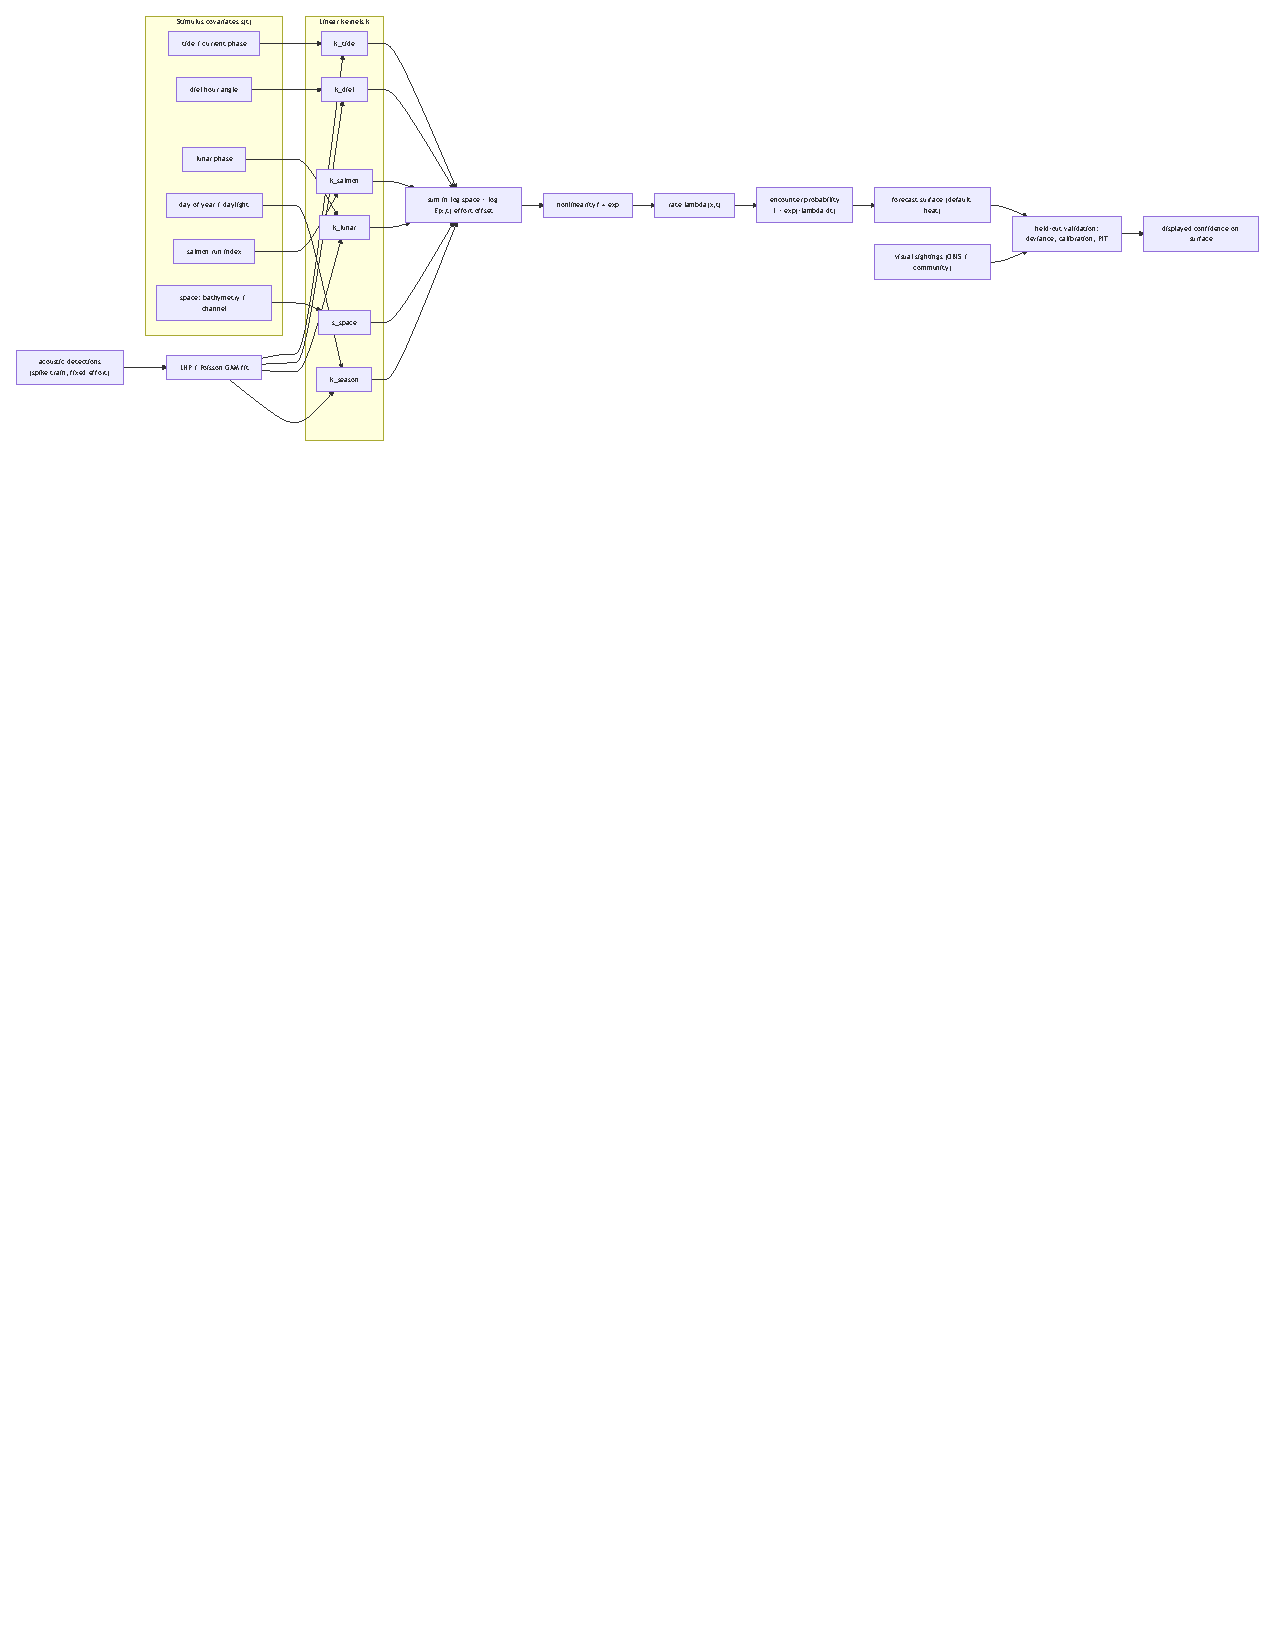
\includegraphics[width=\linewidth]{model_pipeline.pdf}
  \caption{Model pipeline: stimulus covariates drive linear kernels, summed in
  log space with an effort offset, passed through $f=\exp$ to a rate
  $\lambda(x,t)$ and an encounter probability. Acoustic detections fit the
  temporal kernels; visual sightings validate the surface.}
  \label{fig:pipeline}
\end{figure}

\subsection{The kernels and their data}
\begin{table}[ht]
  \centering
  \small
  \begin{tabular}{@{}llll@{}}
    \toprule
    Kernel & Timescale & Data source & Available now? \\
    \midrule
    $k_{\text{tide}}$ & $\sim 6.2$/$12.4$\,h & NOAA CO-OPS 9449880; currents PUG1702 & Yes (stored) \\
    $k_{\text{diel}}$ & 24\,h & computed from timestamp + lon & Yes (on demand) \\
    $k_{\text{lunar}}$ & 29.5\,d & ephemeris (computed) & Yes (on demand) \\
    $k_{\text{season}}$ & annual & computed from date + lat & Yes (on demand) \\
    $k_{\text{salmon}}$ & weeks--seasonal & Albion + DART, climatology fallback & Yes (stored) \\
    $s_{\text{space}}$ & static & bathymetry + sighting density & Partial \\
    \bottomrule
  \end{tabular}
  \caption{Forecast kernels, their covariate timescales, data sources, and
  current availability.}
  \label{tab:kernels}
\end{table}

\section{Instruments and the de-biasing logic}
Visual sightings are presence-only with severe, structured observation bias:
more observers near Lime Kiln, ferry routes, in daylight, and in summer. Naively
fitting $k_{\text{diel}}$ to sightings would learn ``daytime'' because people
watch in daytime; $k_{\text{season}}$ would learn tourism. This is designed out
two ways. First, acoustic data carries the temporal truth: OrcaHello /
Orcasound hydrophones monitor continuously, with effort that does not track human
daylight or tourism, so the temporal kernels are estimated primarily from
continuous acoustic detections at fixed stations where effort $E$ is known and
roughly constant. Second, an explicit effort offset $\log E(x,t)$ enters the
model wherever effort is heterogeneous, so the kernels estimate presence, not
observation. This splits the instrument roles: hydrophones estimate the temporal
kernels; NOAA tides/currents, ephemeris, and the salmon index are the stimulus
covariates; visual sightings (OBIS / community) are held-out validation plus the
social and citizen-science layers. Acoustic presence is not the same as a
visible encounter; the bridge from acoustic $\lambda$ to visible-encounter
probability is an open decision.

\section{The data layer (what is wired)}
\label{sec:data}
Time-series history is stored as S3 partitioned NDJSON under
\texttt{timeseries/\{stream\}/\{station\}/\{yyyy\}/\{mm\}.ndjson}; DynamoDB tables
serve entity / ``latest'' reads. As of 2026-06-19 the data gate is satisfied and
\texttt{/health} reports \texttt{healthy} with 76 normalized sightings.
Table~\ref{tab:data} lists the verified live counts.

\begin{table}[ht]
  \centering
  \small
  \begin{tabular}{@{}lllr@{}}
    \toprule
    Stream / store & Source & Coverage & Records \\
    \midrule
    \texttt{acoustic\_detections} (S3) & OrcaHello (\texttt{haro\_strait}) & 2020-09..2021-04 & $761$ \\
    \texttt{env\_water\_level} (S3) & NOAA Friday Harbor 9449880 & hourly history & $175{,}445$ \\
    \texttt{env\_currents} (S3) & NOAA Rosario Strait PUG1702 & predictions & $17{,}544$ \\
    \texttt{salmon\_run\_index} (S3) & Albion / DART + climatology & daily & $783$ \\
    \texttt{station\_uptime} (S3) & 9 Orcasound stations & accumulating & $27$ \\
    sightings: \texttt{obis\_verified} (DynamoDB) & live OBIS API & live & $248$ \\
    sightings: \texttt{inaturalist} (DynamoDB) & iNaturalist API & live & $5$ \\
    sightings: \texttt{orcahello} (DynamoDB) & OrcaHello & live & $1$ \\
    sightings: \texttt{community} (DynamoDB) & community self-posting & live & $1$ \\
    \bottomrule
  \end{tabular}
  \caption{Live data inventory, verified 2026-06-19. All data-wiring fitness
  gates satisfied.}
  \label{tab:data}
\end{table}

Static assets (committed): \texttt{san\_juan\_land.geojson} (50 island polygons,
OSM coastline) and \texttt{san\_juan\_bathymetry.json} (589 points, NOAA ETOPO1,
depth $-320$ to $+621$\,m). Diel/solar/lunar covariates are computed on demand.
All adapters write through a single \texttt{TimeSeriesStore} abstraction (S3
NDJSON in production, an in-memory mirror for tests): \texttt{put\_series},
\texttt{get\_series}, \texttt{list\_stations}; partitions are merged per month
and deduplicated by $(t, \mathrm{id})$. An EventBridge \texttt{rate(30 min)} rule
invokes a Lambda that makes keyed calls to \texttt{/api/sightings/ingest} and
\texttt{/api/timeseries/refresh}.

\section{Architecture and data flow}
Sources feed adapters, adapters write to the two stores, the API serves status
and ingest endpoints, and the kernel model reads the stores to produce the
forecast surface (Figure~\ref{fig:dataflow}). The public community endpoint and
the EventBridge schedule both write into this pipeline: the public
\texttt{POST /api/community/sightings} writes a citizen-science submission, and
the scheduled service self-writes the time-series streams.

\begin{figure}[ht]
  \centering
  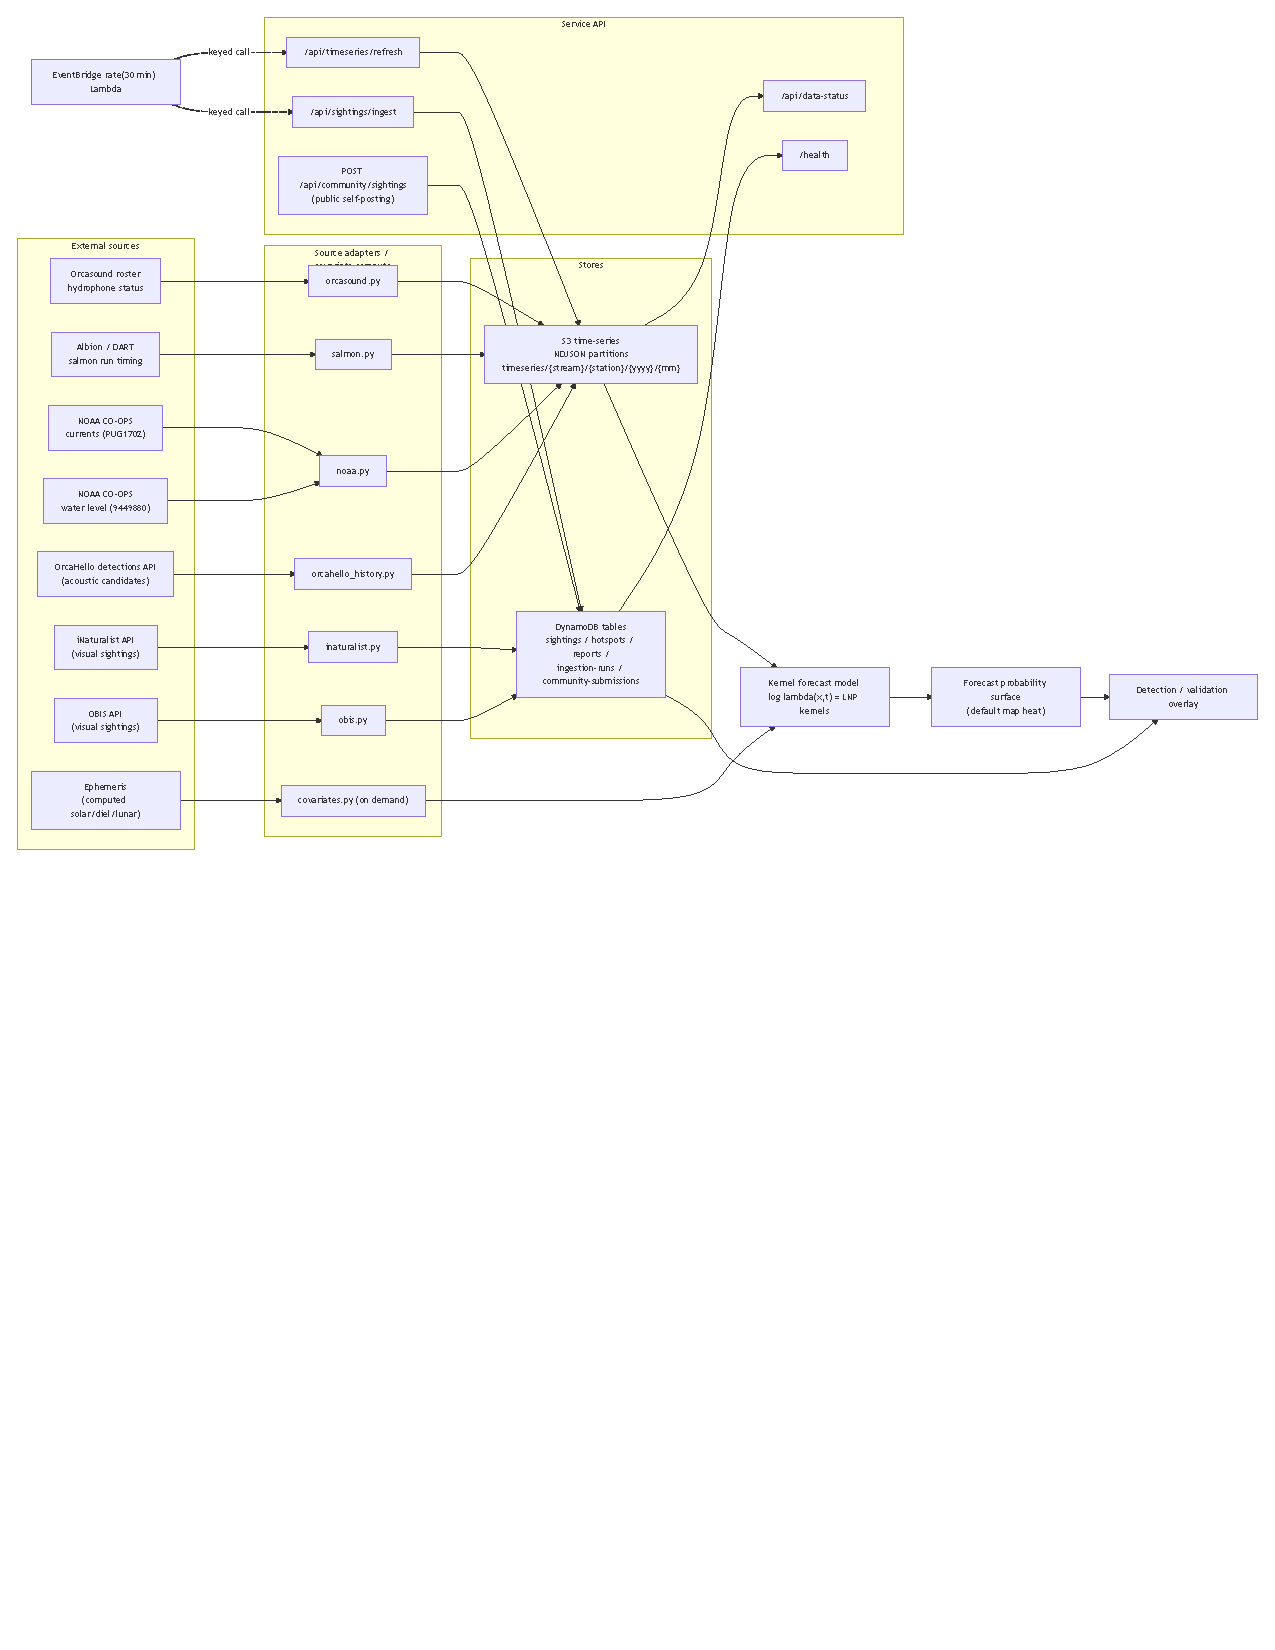
\includegraphics[width=\linewidth]{data_flow.pdf}
  \caption{Data-wiring flow: external sources $\to$ adapters $\to$ S3
  time-series and DynamoDB stores $\to$ service API $\to$ kernel model $\to$
  forecast surface, with the community self-posting endpoint and the EventBridge
  schedule writing into the same pipeline.}
  \label{fig:dataflow}
\end{figure}

\section{Database design and ERD}
Two stores back the system: DynamoDB for entities (each table keyed by
$\texttt{pk} = \texttt{id}$) and the S3 time-series NDJSON store for the
environmental and acoustic streams. The five DynamoDB tables hold
\texttt{NormalizedSighting} (\texttt{orcast-aws-backend-sightings}),
\texttt{Hotspot} (\texttt{-hotspots}), \texttt{ProbabilityReport}
(\texttt{-reports}), \texttt{IngestionRun} (\texttt{-ingestion-runs}), and
\texttt{CommunitySubmission} (\texttt{-community-submissions}).
A \texttt{ProbabilityReport} contains \texttt{Hotspot}s; a \texttt{Hotspot}'s
\texttt{evidence\_sighting\_ids} reference \texttt{NormalizedSighting}s; an
approved \texttt{CommunitySubmission} is adapted into a \texttt{NormalizedSighting}
(\texttt{source = community}); an \texttt{IngestionRun} records a
\texttt{SourceStatus} per source and produces \texttt{NormalizedSighting}s; and
the \texttt{acoustic\_detections} time-series is derived from OrcaHello
(Figure~\ref{fig:erd}).

\begin{figure}[ht]
  \centering
  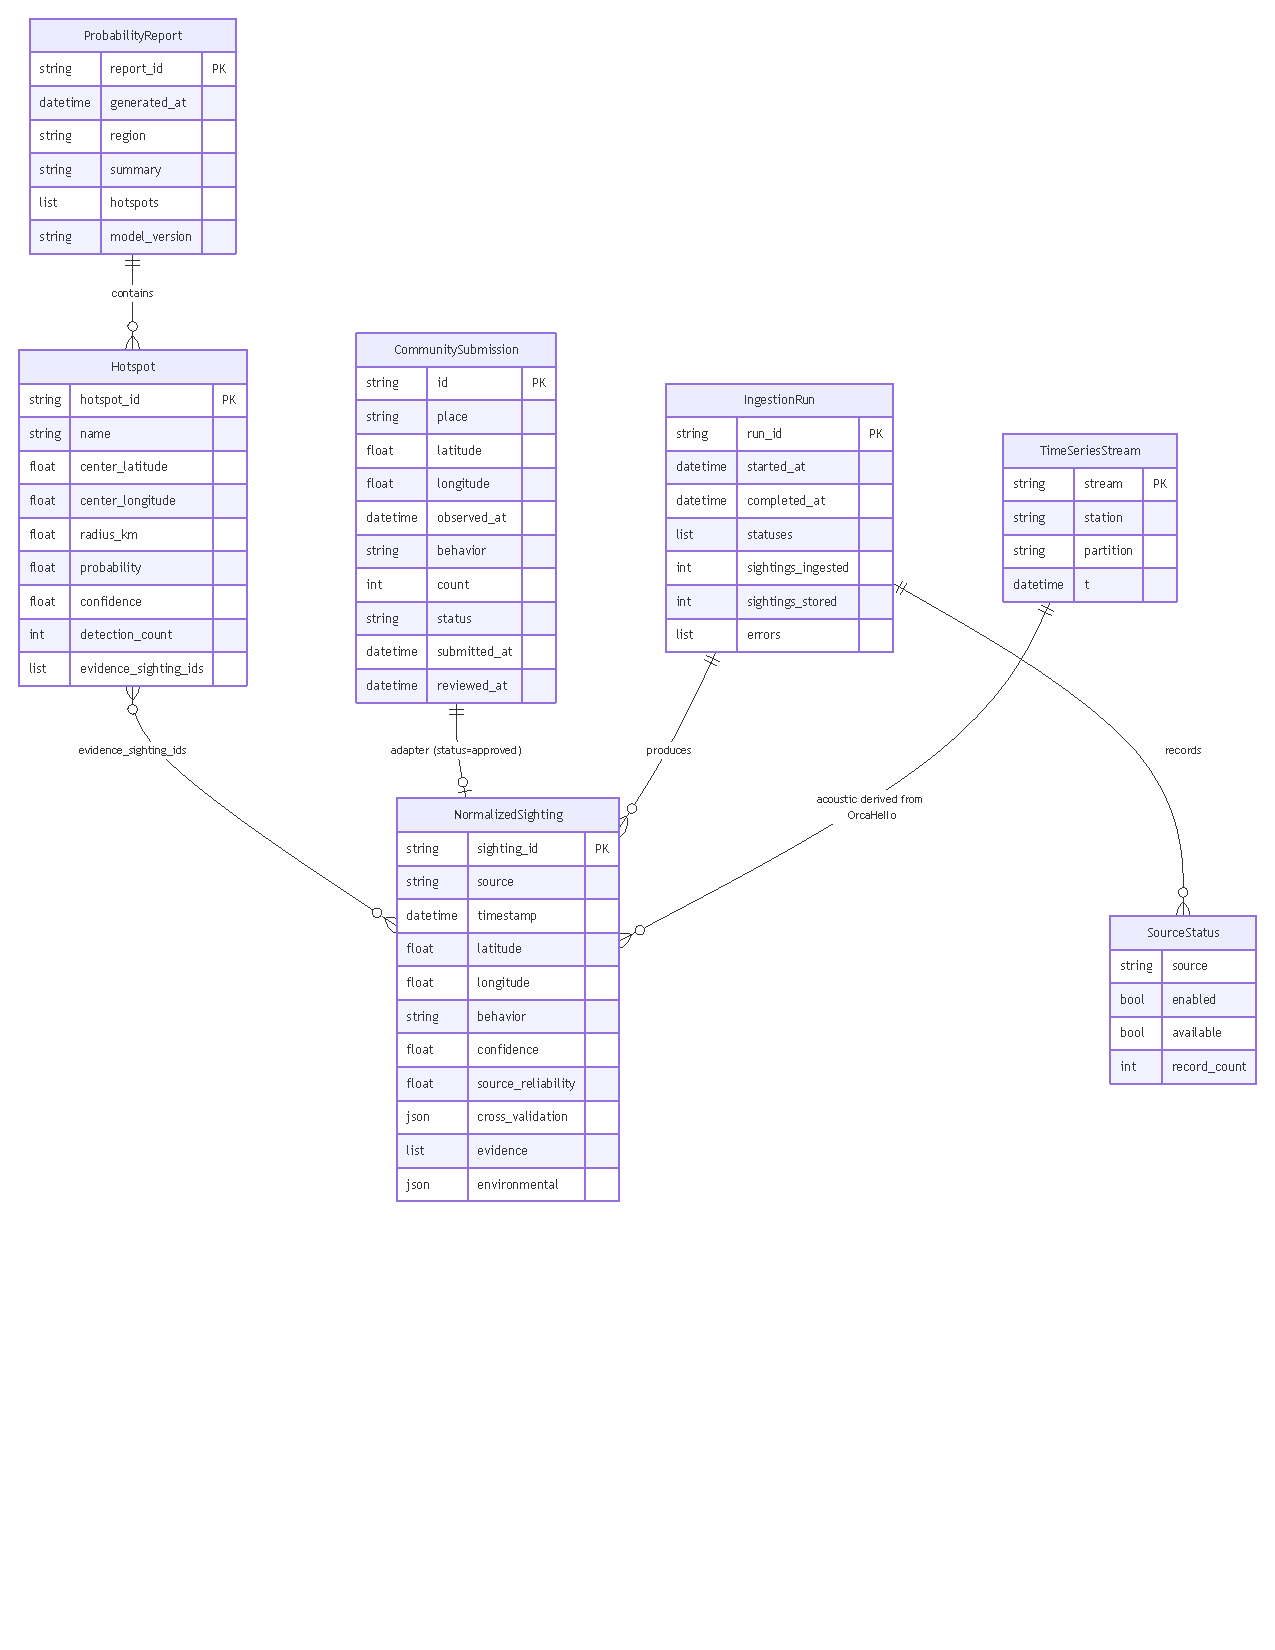
\includegraphics[width=\linewidth]{erd.pdf}
  \caption{Entity-relationship diagram of the five DynamoDB entities, the
  \texttt{SourceStatus} recorded per ingestion run, and the time-series stream,
  with the relationships described in the text.}
  \label{fig:erd}
\end{figure}

\section{Estimation and calibration studies}
\label{sec:calibration}
Recovering a kernel $k$ and a nonlinearity $f$ from a spike train and a stimulus
is exactly the LNP problem, so the kernels are estimated with sensory-neuroscience
methods. Each level states the data it needs and a go/no-go fitness gate; the
forecast is not allowed to sharpen past a level until that level passes on
held-out data, with splits blocked by time (whole cycles held out) to prevent
leakage.

\subsection{Estimation methods}
\begin{enumerate}
  \item \textbf{Peristimulus time histogram (PSTH).} For each cyclic covariate,
  define a repeating stimulus event (sunrise; flood-current onset; new moon;
  Jan~1 / run onset; run peak), align detections to it, bin by phase, divide by
  occupancy/effort, smooth with a periodic spline, and bootstrap cycles for
  confidence bands. The cheapest, most legible first estimate.
  \item \textbf{Reverse correlation / detection-triggered average.} For
  continuous covariates (current speed, tide height, temperature), average the
  covariate trajectory in a window around each detection; whitening the covariate
  autocorrelation separates correlated covariates such as tide and current.
  \item \textbf{Joint LNP / Poisson GLM--GAM (the actual estimator).}
  $\log \lambda(\text{station}, t) = b_0 + a_{\text{station}} + \sum_j
  \text{spline}_j(\text{cov}_j(t)) + \log E(\text{station}, t)$, with penalized
  cyclic splines, station random effects, and an effort offset, fit by penalized
  likelihood or with GP/spline priors. The fitted splines are the kernels and
  should match the PSTH/STA shapes.
\end{enumerate}

\subsection{Leveled plan with fitness gates}
\begin{table}[ht]
  \centering
  \small
  \begin{tabular}{@{}llp{6.4cm}@{}}
    \toprule
    Level & Goal & Fitness gate \\
    \midrule
    L0 & Instrument characterization & Per-station effort series known; detector ROC AUC / $d'$ reported with CI \\
    L1 & Single-covariate PSTH (diel) & PSTH beats a phase-shuffled null; shape consistent across stations \\
    L2 & Joint temporal LNP & Held-out log-likelihood beats climatology and best single covariate; kernels stable across folds \\
    L3 & Prey + space $\to$ field & Held-out skill beats detection-density baseline; calibration within tolerance (PIT $\approx$ uniform) \\
    L4 & Population decoding + uncertainty & Localization validated vs held-out visual sightings; beats persistence; calibration holds out of sample \\
    L5 & Full-confidence forecast & L3--L4 passed; calibration holds; displayed confidence high \\
    \bottomrule
  \end{tabular}
  \caption{Leveled estimation plan. Each gate raises how sharp and confident the
  forecast is allowed to be, not whether it is shown.}
  \label{tab:levels}
\end{table}

\subsection{Sensory-transduction calibration assays}
Beyond fitting, the curves earn trust through assays that probe whether the
response behaves like a real transduction system: dose-response (threshold and
saturation via a Hill-type curve); adaptation/habituation within a presence
bout; signal-detection ($d'$, ROC) for the detector across noise conditions;
null and shuffle controls for every PSTH; cross-validation skill (held-out
deviance, Brier, log-loss vs baselines); reliability diagrams and PIT histograms;
and a population/emergence read-out that treats the network as a distributed
sensor array (per-station LNP units feeding a population decoder), framed as
sensor fusion rather than a claim of cognition.

\section{Roadmap}
\textbf{Phase 0 (now):} data layer wired and validated; covariate library;
instrument-panel overlay UX; forecast shown prior-driven, broad, low-confidence.
\textbf{Phase 1:} fit $k_{\text{diel}}, k_{\text{tide}}, k_{\text{lunar}},
k_{\text{season}}$ from $\geq 1$ year of acoustic (L1--L2); publish kernel curves
with CIs; stand up the validation harness. \textbf{Phase 2:} add
$k_{\text{salmon}}$ and $s_{\text{space}}$; full $\lambda(x,t)$ (L3); backtest vs
baselines. \textbf{Phase 3:} richer uncertainty-aware display and population
decoding (L4); per-ecotype models if labels support it. A \texttt{kernel\_model}
module computes covariates, holds fitted coefficients, and serves $\lambda(x,t)$
grids; fitting runs offline and the service loads coefficients.

\section{Honesty guardrails}
orcast does not run live ML; it consumes the OrcaHello detections API. OrcaHello
records are unreviewed acoustic candidates at a named hydrophone (the unreviewed
stream is dominated by false positives), and a detection's coordinates are the
hydrophone's location, not the animal's. No pod or ecotype identity is shown
unless a source field provides it. External research (Perch~2.0, Palmer~2025,
Pod.Cast, Watkins) is cited as provenance, not presented as orcast capability.
Licenses are respected (OrcaHello-RAIL for the model; CC BY-NC-SA~4.0 for
Orcasound open data; orcast is non-commercial). The forecast is shown honestly,
not hidden: the fitness gates raise its confidence, they do not flip a visibility
switch, and the validation overlay is always available so the forecast can be
checked against observed detections.

\end{document}
